\documentclass{article}
\usepackage[margin=1in]{geometry}
\usepackage{amsmath,amsthm,amssymb}
\usepackage{bbm,enumerate,mathtools}
\usepackage{tikz,pgfplots}
\usepackage{chessboard}
\usepackage[hidelinks]{hyperref}
\usepackage{multicol} % Problem 35

\newenvironment{question}{\begin{trivlist}\item[\textbf{Question.}]}{\end{trivlist}}
\newenvironment{note}{\begin{trivlist}\item[\textbf{Note.}]}{\end{trivlist}}
\newenvironment{references}{\begin{trivlist}\item[\textbf{References.}]}{\end{trivlist}}
\newenvironment{related}{\begin{trivlist}\item[\textbf{Related.}]\end{trivlist}\begin{enumerate}}{\end{enumerate}}


\begin{document}
\rating{4}{1}
A polyform counting problem from Alec Jones: let $a_k(n)$ count the number of polyabolos with $n$ faces
and $k$ exposed edges.
\begin{figure}[!h]
  \centering
  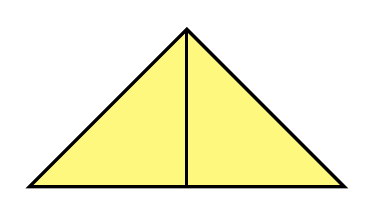
\begin{tikzpicture}[scale=2]
    \draw[very thick, fill={yellow}, fill opacity=0.5] (0,0)--(2,0)--(1,1)--cycle;
    \draw[very thick] (1,1)--(1,0);
  \end{tikzpicture}\hspace{1cm}
  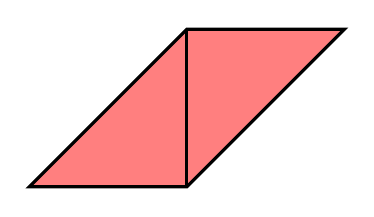
\begin{tikzpicture}[scale=2]
    \draw[very thick, fill={red}, fill opacity=0.5] (0,0)--(1,0)--(2,1)--(1,1)--cycle;
    \draw[very thick] (1,1)--(1,0);
  \end{tikzpicture}
  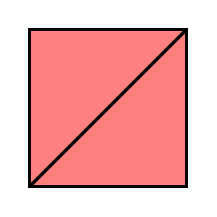
\begin{tikzpicture}[scale=2]
    \draw[very thick, fill={red}, fill opacity=0.5] (0,0)--(1,0)--(1,1)--(0,1)--cycle;
    \draw[very thick] (0,0)--(1,1);
  \end{tikzpicture}\hspace{1cm}
  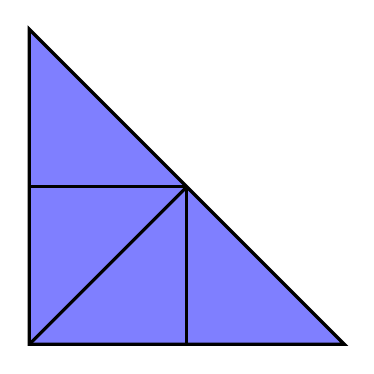
\begin{tikzpicture}[scale=2]
    \draw[very thick, fill={blue}, fill opacity=0.5] (0,0)--(2,0)--(0,2)--cycle;
    \draw[very thick] (0,1)--(1,1);
    \draw[very thick] (0,0)--(1,1);
    \draw[very thick] (1,0)--(1,1);
  \end{tikzpicture}
  \caption{
    An example in yellow showing that $a_3(2) \geq 1$,
    two examples in red showing that $a_4(2) \geq 2$, and
    an example in blue showing that $a_3(4) \geq 1$.
  }
\end{figure}
\begin{question}
  What is the smallest $k$ such that for some fixed $n$, $a_k(n) > 0$?
\end{question}
\begin{related}
  \item What is the largest $k$ such that for some fixed $n$, $a_k(n) > 0$?
  \item What if $\hat{a}_k(n)$ counts polyiamonds instead?
  \item What if concave polygons are excluded?
  \item Is the following function well-defined? \[
    b(k) = \max \{\,a_k(n) : n \in \mathbb{N} \,\}
  \]
  \item Is the following function interesting? \[
    c(n) = \max \{\,a_k(n) : k \in \mathbb{N} \,\}
  \]
\end{related}
\begin{references}
  \item \url{https://en.wikipedia.org/wiki/Polyiamond}
  \item \url{https://en.wikipedia.org/wiki/Polyabolo}
\end{references}

\end{document}
